\chapter{Условные знаки на морских картах и сигналы рейдовых постов}\label{app:2}

\section{Навигационные опасности}\label{app:2a}

\small
\begin{longtable}{M|m{0.2\textwidth}|M|m{0.2\textwidth}}
  \toprule
  \includegraphics[scale=1.3]{APP-2-A-1} & а) камни надводные \newline б) камни надводные на некоторых картах иностранных вод &
  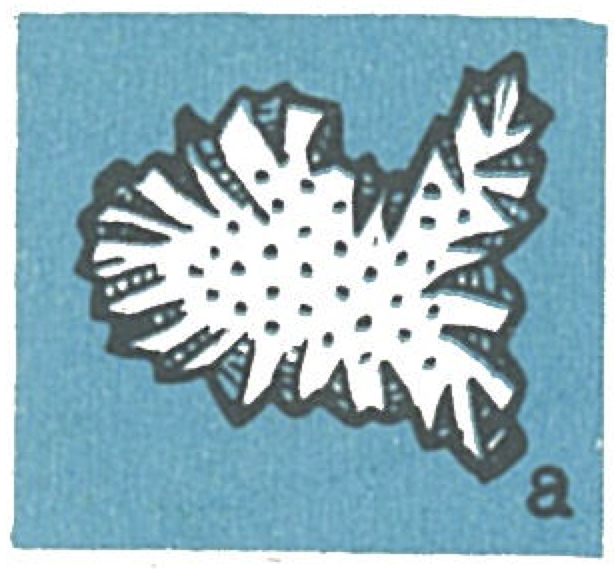
\includegraphics[scale=1.3]{APP-2-A-9} & Рифы осыхающие \newline а) на картах крупных масштабов \\
  \midrule
  
\includegraphics[scale=1.3]{APP-2-A-2} & Камни и скалы подводные и скалы находящиеся на одном уровне с малой водой ($3_8$м \--- глубина над камнем и скалой) &
  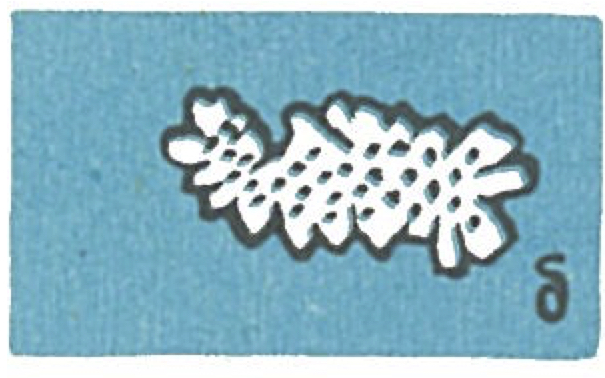
\includegraphics[scale=1.3]{APP-2-A-10} & б) на картах мелких масштабов \\
  \midrule
  
\includegraphics[scale=1.3]{APP-2-A-3} & Камни осыхающие и камни, находящиеся на одном уровне с полной водой ($1_3$м \--- высота осыхания) &
  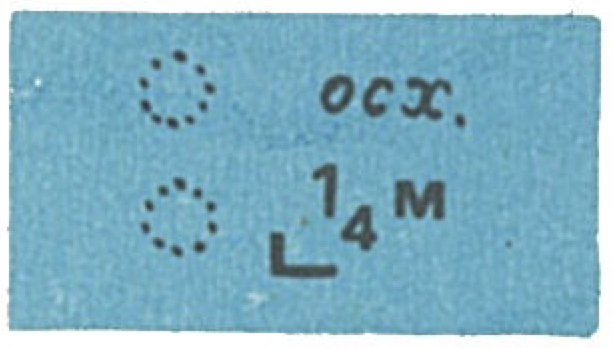
\includegraphics[scale=1.3]{APP-2-A-11} & Осушки, состоящие из мягких пород и не выражающиеся в масштабе карты ($1_4$м \--- высота осыхания)\\
  \midrule
  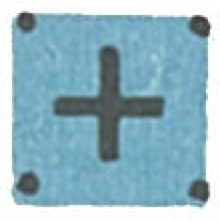
\includegraphics[scale=1.3]{APP-2-A-4} & Буруны &
  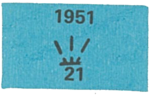
\includegraphics[scale=1.3]{APP-2-A-12} & Места подводных вулканических извержений и выходы горячих газов (1951 \--- год; 21м \--- глубина) \\
  \midrule
  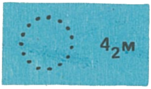
\includegraphics[scale=1.3]{APP-2-A-5} & Банки\index{банка}, не выражающиеся в масштабе карты ($4_2$м \--- глубина над банкой) &
  \includegraphics[scale=1.3]{APP-2-A-13} & Водоросли \\
  \midrule
  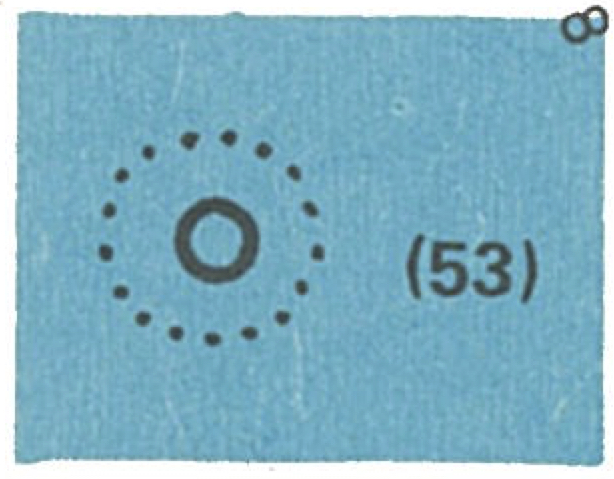
\includegraphics[scale=1.3]{APP-2-A-6} &  Отдельные острова и надводные скалы, не выражающиеся в масштабе карты (53 \--- высота острова или скалы) &
  \includegraphics[scale=1.3]{APP-2-A-14} & Подводные препятствия ($5_4$ \--- глубина над препятствием; $0_9$ \--- высота осыхания ) \\
  \midrule
  \includegraphics[scale=1.3]{APP-2-A-7} & Рифы подводные и рифы, находящиеся на одном уровне с малой водой \newline а) на карте крупных масштабов &
  \includegraphics[scale=1.3]{APP-2-A-15} & Предметы (монолиты, корпуса ботов и т.\=,п.) затопленых в целях рыболовста \\
  \midrule
  \includegraphics[scale=1.3]{APP-2-A-8} & б) на картах мелких масштабов &
  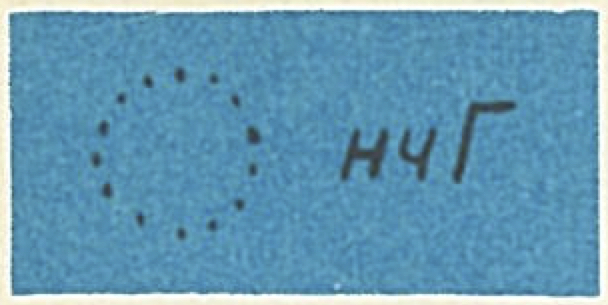
\includegraphics[scale=1.3]{APP-2-A-16} & Районы нечистого грунта \\
  \midrule
  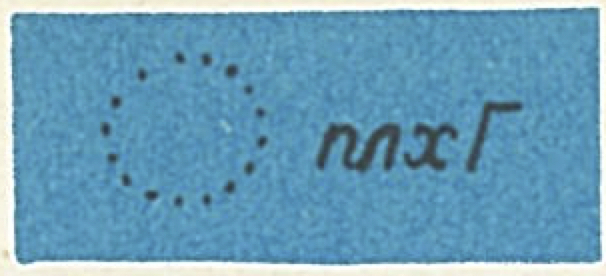
\includegraphics[scale=1.3]{APP-2-A-17} & Плохой грунт (слабо держит якорь) \\
  \bottomrule
\end{longtable}

Точечным пунктиром на карте оконтурены камни, положение которых определено. На некоторых картах иностранных вод оконтурены подводные камни, представляющие опасность для навигации.

У коралловых рифов на картах дано условное обозначение <<Кор>>. Условный знак выходит из употребления.

\small
\begin{longtable}{M|m{0.2\textwidth}|M|m{0.2\textwidth}}
  \toprule
  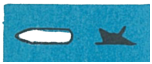
\includegraphics[scale=1.3]{APP-2-A-18} & Затонувшие суда: \newline а) с частями корпуса над водой; &
  \includegraphics[scale=1.3]{APP-2-A-26} & Навигационные опасности, нанесенные (1931 \--- год донесения) \\
  \midrule
  \includegraphics[scale=1.3]{APP-2-A-19} & б) с мачтами над водой; &
  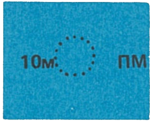
\includegraphics[scale=1.3]{APP-2-A-27} & Подводные мишени (10м \--- глубина над мишенью) \\
  \midrule
  \includegraphics[scale=1.3]{APP-2-A-20} & в) с глубинами над ними 18~м и менее ($12_6$ \--- глубина над затонувшим судном); \newline г) с глубинами над ними более 18м (1941 \--- год гибели судна); &
  \includegraphics[scale=1.3]{APP-2-A-28} & Подводные мишени звуковые (3 \--- количество мишеней, 10\otdo 20м \--- минимальная и максимальная глубина над мишенями) \\
  \midrule
  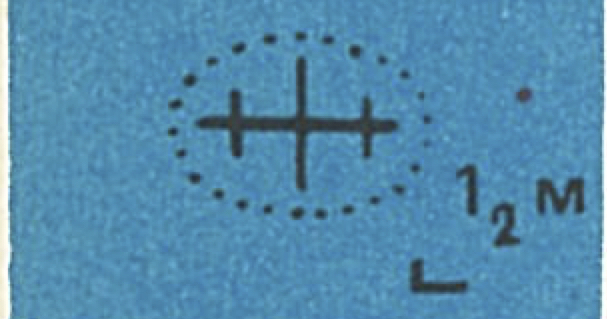
\includegraphics[scale=1.3]{APP-2-A-21} & д) осыхающие ($1_2$м \--- высота осыхания) &
  \includegraphics[scale=1.3]{APP-2-A-29} & Рыболовные сети и заколы \\
  \midrule
  
\includegraphics[scale=1.3]{APP-2-A-22} & Глубина траления над навигационными опасностями: \newline а) без указания способа траления &
  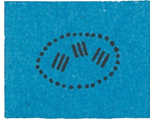
\includegraphics[scale=1.3]{APP-2-A-30} & Скопление топляков и карчей (на картах внутренних водных путей) \\
  \midrule
  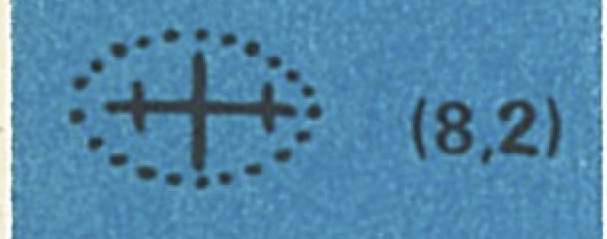
\includegraphics[scale=1.3]{APP-2-A-23} & б) протравлено гибким тралом; &
  \includegraphics[scale=1.3]{APP-2-A-31} & Скопление подводных камней (огрудки) \\
  \midrule
  \includegraphics[scale=1.3]{APP-2-A-24} & в) протравлено жестким тралом &
  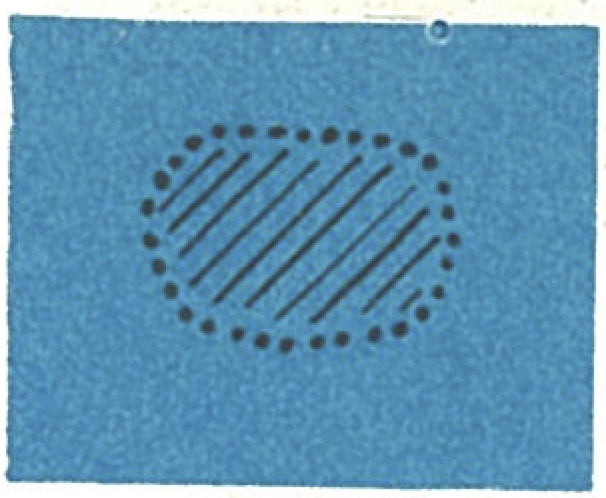
\includegraphics[scale=1.3]{APP-2-A-32} & Затопленный лес \\
  \midrule
  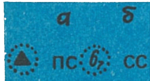
\includegraphics[scale=1.3]{APP-2-A-25} & Навигационные опасности положение (а) или существование (б) сомнительно &
  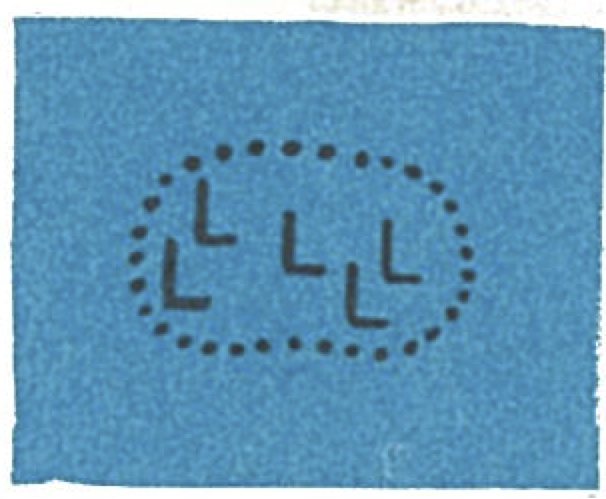
\includegraphics[scale=1.3]{APP-2-A-33} & Затопленные вырубки \\
  \midrule
  
\includegraphics[scale=1.3]{APP-2-A-34} & Зоны всплывшего торфа &
  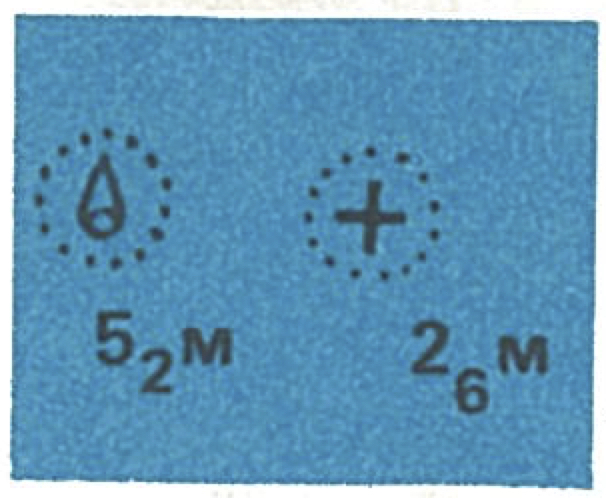
\includegraphics[scale=1.3]{APP-2-A-35} & Затопленные объекты (вышки, церкви и т.\=,п.) ($5_2$ и $2_6$ \--- глубины над объектами) \\
  \bottomrule
\end{longtable}

\section{Береговые средства навигационного оборудования}\label{app:2b}

\small
\begin{longtable}{M|m{0.2\textwidth}|M|m{0.2\textwidth}}
  \toprule
  \includegraphics[scale=1.3]{APP-2-B-1} & Маяки и светящиеся знаки с огнями кругового освещения &
  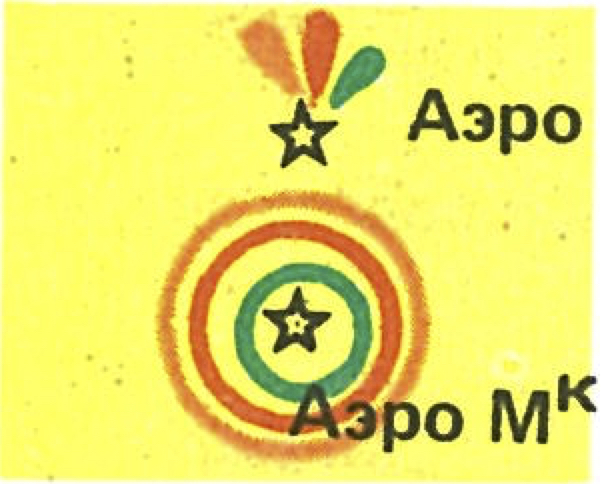
\includegraphics[scale=1.3]{APP-2-B-6} & Аэромаяки с переменными огнями кругового освещения \\
  \midrule
  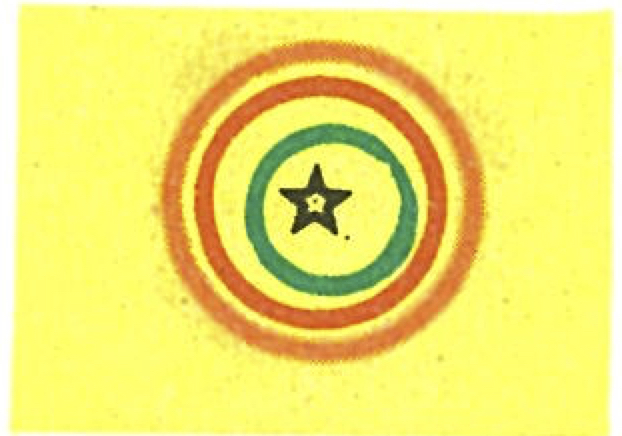
\includegraphics[scale=1.3]{APP-2-B-2} & Маяки и светящие знаки кругового освещения с переменными огнями &
  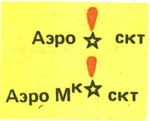
\includegraphics[scale=1.3]{APP-2-B-7} & Аэромаяки с секторными огнями \\
  \midrule
  \multicolumn{2}{c|}{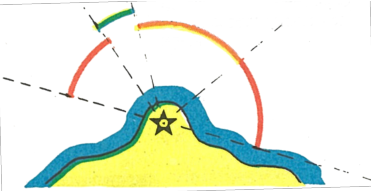
\includegraphics[scale=1.3]{APP-2-B-3}} & 
  \multicolumn{2}{M}{Маяки и светящиеся знаки с секторными огнями} \\
  \midrule
  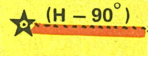
\includegraphics[scale=1.3]{APP-2-B-4} & Направленные огни маяков и светящихся знаков (Н\--90\gr \--- направления, по которому светит сильный свет) &
  \includegraphics[scale=1.3]{APP-2-B-8} & Портовые, рыбацкие и другие огни: \\
  \midrule
  \includegraphics[scale=1.3]{APP-2-B-5} & Аэромаяки с огнями кругового освещения &
  \includegraphics[scale=1.3]{APP-2-B-9} & а) огни, расположенные по вертикали \newline б) огни, расположенные по горизонтали \\
  \midrule
  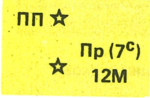
\includegraphics[scale=1.3]{APP-2-B-10} & Маяки, светящиеся знаки и аэромаяки, положение которых на карте приближено &
  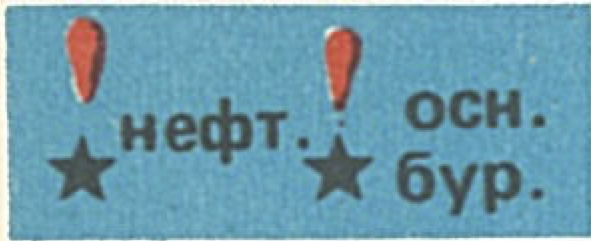
\includegraphics[scale=1.3]{APP-2-B-11} & Огни на сооружениях (нефтяных вышках, основаниях буровых вышек и т.\=,п.) \\
  \midrule
  
\includegraphics[scale=1.3]{APP-2-B-12} & Предостерегательные огни (на нефтяных вышках, основаниях буровых вышек и т.\=,п.) &
  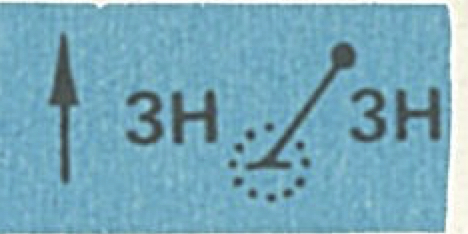
\includegraphics[scale=1.3]{APP-2-B-18} & Стационарные вехи (укреплённые в грунте) \\
  \midrule
  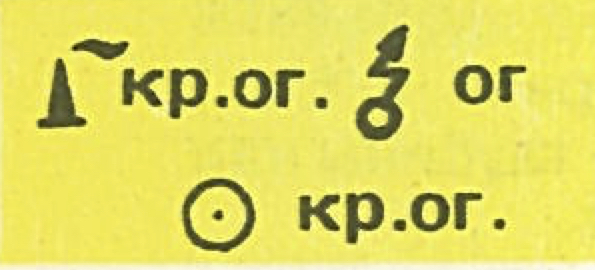
\includegraphics[scale=1.3]{APP-2-B-13} & Заградительные авиационные огни &
  \includegraphics[scale=1.3]{APP-2-B-19} & Предостерегающие надписи \\
  \midrule
  \includegraphics[scale=1.3]{APP-2-B-14} & Несветящие навигационные знаки (20,3 \--- высота от принятого нуля высот, 7 \--- высота от основания до вершины знака) &
  \includegraphics[scale=1.3]{APP-2-B-20} & Теплопеленгаторные станции \\
  \midrule
  \includegraphics[scale=1.3]{APP-2-B-15} & Гурии &
  \includegraphics[scale=1.3]{APP-2-B-21} & Ведущие кабели \\
  \midrule
  \includegraphics[scale=1.3]{APP-2-B-16} & Знаки, ограждающие подводные кабели, трубопроводы и т.\=,п. &
  \includegraphics[scale=1.3]{APP-2-B-22} & Акустические средства: \newline а) звукосигнальные установки; \\
  \midrule
  \includegraphics[scale=1.3]{APP-2-B-17} & Световые отражатели &
  \includegraphics[scale=1.3]{APP-2-B-23} & б) гидроакустические установки; \newline в) гидролокационные маяки; \newline г) гидролокационные пассивные отражатели \\
  \bottomrule
\end{longtable}

На некоторых картах иностранных вод на знаках показаны топовые фигуры.

\small
\begin{longtable}{m{0.46\textwidth}|m{0.46\textwidth}}
  \toprule
  \includegraphics[scale=1.3]{APP-2-B-25} & \includegraphics[scale=1.3]{APP-2-B-27} \\
  Створы маяков и светящих знаков (90\gr \--- направление створа с берега, 270\gr \--- направление створа с моря) & Створы огней \\
  \midrule
  \includegraphics[scale=1.3]{APP-2-B-26} & \includegraphics[scale=1.3]{APP-2-B-28} \\
  Огни створных маяков и светящих знаков, светящие в узком секторе & Створы несветящих знаков \\
  \midrule
  \includegraphics[scale=1.3]{APP-2-B-29} & \includegraphics[scale=1.3]{APP-2-B-32} \\
  Створы знаков, ограждающих  подводные кабели, трубопроводы и т.\=,п. & Ограничительные створы \\
  \midrule
  \includegraphics[scale=1.3]{APP-2-B-30} & \includegraphics[scale=1.3]{APP-2-B-33} \\
  Прицельные створы & Мерные линии с ведущим створом \\
  \midrule
  \includegraphics[scale=1.3]{APP-2-B-31} & \includegraphics[scale=1.3]{APP-2-B-34} \\
  Щелевые створы. (При плавании по створу средний огонь или знак должны быть видны между крайними огнями или знаками) & Мерные линии с рекомендованным курсом \\
  \bottomrule
\end{longtable}

\section{Плавучие средства навигационного оборудования}%\label{app:2c}

\small
\begin{longtable}{M|m{0.2\textwidth}|M|m{0.2\textwidth}}
  \toprule
  \includegraphics[scale=1.3]{APP-2-C-1} & Плавучие маяки &
  \includegraphics[scale=1.3]{APP-2-C-2} & Буи светящие \\
  \midrule
  \includegraphics[scale=1.3]{APP-2-C-3} & Плавучие огни &
  \includegraphics[scale=1.3]{APP-2-C-4} & Буи несветящие \\
  \midrule
  \includegraphics[scale=1.3]{APP-2-C-5} & Буи с топовыми фигурами &
  \includegraphics[scale=1.3]{APP-2-C-6} & Западные вехи \\
  \midrule
  \includegraphics[scale=1.3]{APP-2-C-7} & Буи над опасностями &
  \includegraphics[scale=1.3]{APP-2-C-8} & Восточные вехи \\
  \midrule
  \includegraphics[scale=1.3]{APP-2-C-9} & Бочки: \newline а) швартовные; \newline б) ограждающие; \newline в) швартовные для гидросамолетов; \newline г) девиационные &
  \includegraphics[scale=1.3]{APP-2-C-10} & Крестовые вехи \\
  \midrule
  \includegraphics[scale=1.3]{APP-2-C-11} & Буи или бочки над подводными мишенями &
  \includegraphics[scale=1.3]{APP-2-C-12} & Вехи разделения фарватеров и каналов, осевые и ограждающие затонувшие суда \\
  \midrule
  \includegraphics[scale=1.3]{APP-2-C-13} & Огни над подводными препятствиями &
  \includegraphics[scale=1.3]{APP-2-C-14} & Флажные вехи \\
  \midrule
  \includegraphics[scale=1.3]{APP-2-C-15} & Огни на затонывших судах &
  \includegraphics[scale=1.3]{APP-2-C-16} & Ледовые вехи. Шесты \\
  \midrule
  \includegraphics[scale=1.3]{APP-2-C-17} & Огни на суда для буровых работ &
  \includegraphics[scale=1.3]{APP-2-C-18} & Светящие вехи \\
  \midrule
  \includegraphics[scale=1.3]{APP-2-C-19} & Северные вехи левой стороны, левые поворотные каналов (фарватеров) &
  \includegraphics[scale=1.3]{APP-2-C-20} & Световые отражатели на буях и вехах \\
  \midrule
  \includegraphics[scale=1.3]{APP-2-C-21} & Южные вехи правой стороны, правые поворотные каналов (фарватеров) &
  \includegraphics[scale=1.3]{APP-2-C-22} & Светоотражающие покрытия на буях и вехах \\
  \midrule
  \includegraphics[scale=1.3]{APP-2-C-23} & Буй-маяк \\
  \bottomrule
\end{longtable}

\section{Радиотехнические средства навигационного оборудования}%\label{app:2d}

\small
\begin{longtable}{M|m{0.2\textwidth}|M|m{0.2\textwidth}}
  \toprule
  \includegraphics[scale=1.3]{APP-2-D-1} & Станции радионавигационных систем &
  \includegraphics[scale=1.3]{APP-2-D-2} & Радиостанции работющие по запросу (требованию пеленгования) \\
  \midrule
  \includegraphics[scale=1.3]{APP-2-D-3} & Секторные радиомаяки дальнего действия &
  \includegraphics[scale=1.3]{APP-2-D-4} & Радиопеленгаторные станции \\
  \midrule
  \includegraphics[scale=1.3]{APP-2-D-5} & Радиомаяки &
  \includegraphics[scale=1.3]{APP-2-D-6} & Радиолокационные маяки (непрерывно излучающие импульсы) \\
  \midrule
  \includegraphics[scale=1.3]{APP-2-D-7} & \multirow{2}{*}{\shortstack[l]{Радиомаяки\\при световых\\маяках}} &
  \includegraphics[scale=1.3]{APP-2-D-8} & Радиолокационные маяки-ответчики \\
  \cmidrule{3-4}
  \includegraphics[scale=1.3]{APP-2-D-9} & &
  \includegraphics[scale=1.3]{APP-2-D-10} & Радиолокационные маяки для калибровки судовых радиолокационных станций \\
  \midrule
  \includegraphics[scale=1.3]{APP-2-D-11} & Радиомаяки на светящихся буях &
  \includegraphics[scale=1.3]{APP-2-D-12} & Береговые радиолоуационные станции \\
  \midrule
  \includegraphics[scale=1.3]{APP-2-D-13} & Аэрорадиомаяки &
  \includegraphics[scale=1.3]{APP-2-D-14} & Радиолокационные станции, имеющие значение только навигационных ориентиров \\
  \midrule
  \includegraphics[scale=1.3]{APP-2-D-15} & Аэрорадиомаяки при аэромаяках &
  \includegraphics[scale=1.3]{APP-2-D-16} & Радиолокационные отражатели \\
  \midrule
  \includegraphics[scale=1.3]{APP-2-D-17} & Радиомаяки и аэрорадиомаяки, положение которых на карте приближенно &
  \includegraphics[scale=1.3]{APP-2-D-18} & Радиолокационные ориентиры \\
  \bottomrule
\end{longtable}

%%% Local Variables:
%%% mode: latex
%%% TeX-master: "yacht-captain.tex"
%%% End:
